\chapter{Concepts} 
\label{ch:concepts}

\section{Github and Git} 
\label{sec:library}

Github and Git together are version control systems which archive information in FOSS communities. Git is used to access Github from the CLI, such as through the set of three commands that move changes to the remote repository, "git add", "git commit", and "git push" \cite{gitdocs}. Github then holds the commits and are brought to other users' local repositories using "git pull", facilitated by the owner of the local repository \cite{gitdocs}. Github also holds records of all the branches that have been pushed to the remote repository, all of the forks made of the main project repository, and all of the releases made of that software. 

Github and Git are included as software applications to study for this thesis because of their importance in software development, especially open source software development. Github includes their own education program, Github Education, that specifically trains users to use their program for building software \cite{githubedu}, in addition to very extensive self-directed documentation in Github Docs \cite{githubdocs}. This is accompanied by documentation for Git as well \cite{gitdocs}. Because Github holds so many vital FOSS communities and projects, and appropriately equipped and documented to support users and contributors, Git and Github are good candidates for study in this thesis. 

\section{The Library} 
\label{sec:library}

The Library is a core concept to this research because it is necessary to understand the qualities of both physical and virtual libraries before applying these concepts to Github and Computer Science. This section explores how the qualities of libraries defined by Gorman and Rubin apply do not apply to Github, factoring in a more broad definition of "the library" for this thesis, influenced by prior definitions for the physical library and the concept of the library. First, it is necessary to determine this definition for the library. 

\subsection{Defining the Library}

\subsubsection{ALA Definition}
According to the ALA, there are three definitions for "library", "1. A collection (5) of materials in various formats (4) organized to provide physical, bibliographic, and intellectual access to a target group , with a staff trained to provide services and programs related to the information needs of the target group . 2. A building or structure that houses such a collection (5). 3. The institution that manages such a collection (5). 4. A private collection (3) of materials , often owned by an individual, such as books , sound discs, or videodiscs." \cite{glossary2013}. These definition seems to be more focused on either the physical library as a location or the tangible parts of the library. Although this still applies to the first and last definition, both mention collections of information, and the first mentions additional resources the enable access to information. Therefore, the information itself and these related resources seem to be the two most important parts of the definition of a library. 

\subsubsection{Malczewski's Definition}
In \textit{Foundations of Library and Information Science: Fourth Edition} Rubin quotes Malczewski's goes beyond the physical components of the "library", "A library building is more than a container for content, digital or print. It is a cultural space recognized as a place of learning. Its presence in a community is both practical and symbolic: "The library has often, and for obvious reason, become synonymous with reading and literacy, but the true definition of the library has always been ideological and transcendent of format: to inspire, facilitate learning, to advance knowledge, and to strengthen the community. In this, a library’s space is different from that of a warehouse, as it has values, a philosophy, a spirit, and a soul. Not just a personalized space, it is personified as a lexicon of local culture and the human experience." (Malczewski 2014, p. 37)". \cite{rubin2016foundationslis} \cite{malczewski2014meaningful}. Malczewski's definition focuses more on the philosophical definition of the library. For this thesis, there is certainly value in the reading of written code and literacy of code, which will be further elaborated later in this chapter. An important part of this definition seems to be the inclusion of "culture" and "community", which indicate how the library is more than a simple collection of information. 

Github embodies both ends of these different definitions of the library because it is a platform which allows access to massive collections of information, holds these collections, and can direct users to this information. Github is also a space that is central to the FOSS community, and facilitates this collaboration and the culture within directly through this platform. 

\subsection{Gorman's Core Values}

\subsubsection{Stewardship}

Gorman's first value Stewardship, defined as "“preservation of the human record to ensure that future generations know what we know, care and nurture of education for librarianship so that we pass on the best professional values and practices, the care and maintenance of our libraries so that we earn the respect of our communities" \cite{gorman2000values}. In elaborating on Stewardship, Gorman stresses the importance of physical record keeping of information continuing even as technology advances. This argument supports the the inclusion of Github in the library catalog. Even if there is not printed code in the books within the library, the librarians who are within the physical library would have knowledge of the code that can be accessed directly through the online library catalog. One of Gorman's central concerns in the book seems to be the erasure of the physical library in place of a fully online library. This research does not argue for the library to move fully online, rather the physical library and it's virtual (fully virtual or both physical and virtual) should continue to coexist. 

Gtihub allows for the preservation of the code, which has certainly become part of the "human record" as technology advances and becomes a central part of society today. This preservation is enabled through the use of Git, an application with which Github users can add or "push" new or updated material to Github, and "pull" or retrieve material from Github that is not on their local machine. On the Github website view of the repository, there is a commit log kept of all versions of this repository that have been pushed to the platform. A complication of this record keeping is the potential for either the user or Github to have incomplete versions of the repository. If the user does not consistently pull from a repository, especially if this repository is pushed to by many users, the record on their local machine will lack some of the information on the Github record. Additionally, if the user makes changes to their local repository but does not push these changes to Github, the record on Github is incomplete. If the repository is shared with other users and they pull the information, then their local record is incomplete. The best practice for keeping the local repository up to date is to push and pull often, specifically pushing for each line in code changed. This practice is not as well defined for documentation beyond code files, as changes could be several lines long, and pushing for each individual line could be impractical. 

Github does not have an organized form of education related to the platform, however, documentation might be considered a form of education. Documentation is used to communicate the necessary information to aid users in contributing to Github. Whereas the education Gorman describes is more direct, with librarians interacting with patrons to teach them, the Github documentation is more individualized, where users are free to consult that information as they need, without the direct aid of another human. In the case of Github, the educational aspect is far more self-directed. 

There are several different forms of documentation on Github. A vital part of Github is their Git Flow, which is a best practice for contributing to a repository in a logical, organized manner. There is documentation written by Github which explains each step of the Git Flow, from start to finish. There is also documentation for the use of Markdown, a language used to write documentation. This is used specifically in the README.md file, which acts as a front page to the repository and usually contains the necessary information to understand what the repository holds, it's purpose, who has contributed to the project, and if the project accepts contributions. The CONTRIBUTING.md file may be linked here, which holds the guidelines for contributing to the repository and has recently become a best-practice for repositories that accept contributions. 

A concern Gorman includes in the argument for Stewardship is in an increasingly online world is the "trust between author, publisher, and reader", “There is nothing to stop anyone from gaining access to any electronic document and changing it to his or her heart’s delight before disseminating it as something it is not. That is the heart of the dilemma faced by authors and readers in an electronic world devoid of of fixity, standardization, and verifiable veracity” \cite{gorman2000values}. In the case of Github and Git Flow, the ability for anyone to make changes to open source software is incredibly vital to the advancement and maintenance of software. However, in repositories with maintainers, Git Flow is a standardization which helps to maintain the integrity of the software and project. Once the user has made changes to the fork or branch that meet their goals own goals for contributing to the project, they are able to open a pull request and request for the maintainers of the repository to review their work. In the review, the maintainers have the ability to accept the work as it is and merge the new changes and additions into the software, or request changes from the user before the merge can be completed.

Lastly, Gorman discusses the enormous task of preserving all resources online and making sure they are preserved in all forms, including unmodified forms. Again, Git and Github support this through the Git Flow action of forking to contribute to a repository and holding commit history of all the changes made, However, as discussed previously with preservation, the commit history and versions which exist depend upon how often commits have been created, and if they have been pushed to Github. 

\subsubsection{Service}

Service is defined as  “duty done or required, professional or other useful ministrations, effort inspired by philanthropic motives or dedicated to human welfare or embetterment” \cite{gorman2000values}. Because the choice to participate in contributing on Github is entirely voluntary, the value of Service is somewhat supported in understating Github through Library Science concepts, though this is limited. Although maintainers may feel they are required to complete work in the repository, the choice to be a maintainer is entirely voluntary. At any point, a maintainer could choose to leave a project, although it should be handed to another maintainer first so that it is not abandoned. This is one of the options Raymond gives in \textit{Homesteading the Noosphere} for how projects change ownership, and the only option where the projects remains active and actively maintained \cite{raymondnoosphere}. However, it is still possible for a project to be abandoned if that it what the maintainer chooses. Overall Service as it applies to Github would apply to the maintainers as they carry out their responsibilities. 


\subsubsection{Intellectual Freedom}

Intellectual Freedom in how it is discussed by Gorman does not apply to Github in most cases. The listed qualities that make up intellectual freedom are "“commitment to the idea that all people should be able to read and see whatever they wish to read and see, defending intellectual freedom of all community members, defending free expression of minority opinion, and making facilities and programs accessible”\cite{gorman2000values}. Because Github is such an individualized platform, there is not a "commitment" or "defending" of this idea on Github. The only limitations of information being included on Github as a whole would be those which violate Github's Terms of Service. Within the repositories, the inclusion of information would depend upon on which pull requests the maintainers choose to accept, and changes which they request from the author of the pull request. This process would depend on the choices of the maintainers on what should be included in the project, which would be more focused on the needs of building the project or addressing bugs rather than "free expression". 

Accessibility in the context of intellectual freedom is more focused on the ability to access information without ideological limitations preventing access, rather than technical or monetary barriers, such as paid accounts or not having access to a computer from home. This understanding of accessibility may be supported by the nature of open source software being available for free use. Because of this, Open Source Software on Github is in public repositories which allow anyone to view the source code and download the repository to use the software. 

\subsubsection{Rationalism}

The definition given for Rationalism is "“The philosophical belief that reason is a source of knowledge in itself-independent of emotions, faith, and the senses-is the basis for the rational approach", further characterized by the organization of the library, instructing rationally to educate people to have a similar basis in their approach and “bibliographic control” \cite{gorman2000values}. This idea is applicable to the organization of the Github repository, and the use of Git Flow. Rationalism seems to rely on logic to govern organization and operations, which is reflected in the overall repository structure, the actions this enables, and the Git Flow model. 

The base repository structure is uniform across all Github repositories, with tabs in this order, left to right: Code, Issues, Pull Requests, Actions, Projects, Wiki, and Security. The Code tab is the main page of the repository, which displays the READEME file below a list of the repository's file system and the most recent commit, which links to the commit history of the repository. The Issue Tracker tab shows all open issues, and can be searched, including for specific labels and closed issues. The labels can be used to differentiate the purpose of the issue, such as proposing a new feature or noting a bug that needs solved. Actions include automation that can be used to aid maintainers in their work, such as bots which close "stale" pull requests, which have had no activity after a certain amount of time. The Projects tab allows maintainers to create interactive project boards to track past, current, and future tasks, and is able to be viewed by contributors working on the project. 

\subsubsection{Literacy and Learning}

The qualities which Gorman defines to represent Literacy and Learning are "encouraging literacy and a love of learning, encouraging lifelong sustained reading, and making the library a focus of literacy teaching"\cite{gorman2000values}. Again, because participation Github and contributing to software is such an individualistic process, this complicates how Github might encourage literacy or continuous education. That encouragement is not consistently part of Github, although there are events which do encourage that participation. An example of this would be Hacktoberfest, which is a hackathon hosted on Github in collaboration with DigitalOcean. There are free t-shirts offered to partcipants who complete a set number of pull requests in public repositores during the month of October. However, this is an isolated event that is not consistently part of Github. Additionally, the core purpose of Github is to hold information, not to teach programming. The documentation necessary for learning how to use and contribute to software is typically made available to read in the associated repository, or on the website for the tool in the case of Git. However, it is up to the individual to consult this information, rather than Github consistenly encouraging contributors to do so. This is the same case for "sustained reading" - it is the individual's choice, although it is best practice to read the new documentation for new versions of software, especially if significant changes have been made since the prior version. 

On the idea of Literacy, Gorman writes, "Literacy is not just a question of reading and writing, even at the highest level, but also an ability to express oneself fully", and "Some see the three abilities (reading, writing, and speech) as inextricably intertwined. I think that reading is the central portion of this complex in that one could live the life of the mind in isolation with printed texts...whereas it is safe to say, writing is well impossible for someone who does not read"\cite{gorman2000values}. Gorman argues for the importance of reading in literacy. Although a core purpose of Github is not to cultivate literacy of code, the access to code that is provided by Github allows for individuals to read through code and documentation to further understand how the code functions. This could be limited by prior knowledge of repository structure, as it is often necessary to find the folder where the main code is held. Approaching this from a Library Science perspective, since Github does not inherently include literacy efforts, librarians and technical resources that are available in the physical library could be applied in addressing literacy of code. 

\subsubsection{Equity of Access}
Access to Github as a whole is dependent upon the user's ability to access both an internet connection and an electronic device. It is possible to access Github on a phone, but access via a computer or tablet which includes a command-line interface is more user-friendly as it allows for interaction with the full Git Flow process of pushing and pulling from the local version of the repository. Not everyone has access to WIFI or access to a computer at home, which would require more effort to access Github to the same level as those who have the means to access this from home. To some extent, it is possible to increase the equity of access through physical libraries, however this is an incomplete solution because this still requires transportation to the library and availability during library open hours, and limits access to Github to only those when the library is open.  Once a user has access to an internet connection and a computer, there is no cost associated with creating an account on Github, searching through the repositories, and contributing to them. 

A complication specific to Github itself is the pro account upgrade, which costs four dollars per month and totals forty eight dollars per year. This type of account seems to be more oriented toward developers rather than providing more access to Github as a whole, but it allows users with this account to create private repositories that only they can access. Private repositories could limit access to code and information for other users, potentially creating issues of access. Users with free accounts and users with paid accounts are both able to access the massive number of repositories on Github, but this is complicated by the inability for users to access private repositories that are not under their account. 

Because access to Github is dependent upon access to internet and a computer, and although accounts are free, there are paid accounts that allow private repositories, Github does have some level of Equity of Access. There is not a absence of this because of the ability to create a free account, but it is not to the same level of a physical library because there are private repositories and a private account upgrade which allows for more privacy than a free account and blocks open access to information for other users. 

\subsubsection{Privacy} 

A large portion of Gorman's description of how privacy should function in a library focuses on the privacy of library records, including circulation records \cite{gorman2000values}. On Github, all circulation records are public except for those in private repositories. This is necessary to best support Github's purpose as a center of collaboration for open source communities. If a user would prefer that their participation in circulation remains private, they are able to use a private repository, but the options for limiting visibility when contributing to public repositories is limited. This could occur if multiple commits, including their own, are squashed into one single commit by another user and pushed to the repository by that other user. Any commits made directly by a user will show in the commit history. 

\subsubsection{Democracy}

The value of Democracy does not apply to Github. Gorman's discussion of Democracy as a value includes education about democracy, and Github is used by an international community which includes people who do not live in a country with a democratic government. Additionally, Democracy is not apparent in how Github functions. The maintainers of repositories are not elected by contributors, rather the maintainers may have started the repository and have become a maintainer because of this. The functionality of Github is far more focused on individual choice to participate than collective participation, and there are not elections for choosing individuals who are in a place of power, such as maintainers. 

\subsubsection{Gorman's Qualities of Virtual Libraries}

An interesting point Gorman makes in discussing the implementation of virtual libraries is the funding of the physical library in schools, "Politicians and computer scientists press for schools to be wired to give all schoolchildren access to the Net and the Web, but ignore the underfunded libraries in those same schools and the negative effect of such neglect on reading and the literacy levels of those schoolchildren. Futurists predict that electronic technology will supplant "the book" sooner rather than later, but ignore the fact that technology has made the book production and high production values quicker, easier, cheaper, and more accessible" \cite{gorman2000values}. Throughout \textit{Our Enduring Values} Gorman argues for the preservation of the physical library and warns of the consequences for information if all records were to be virtual in the future. However, as the world becomes increasingly digital, it is necessary for there to be a balance between technological advancements and the preservation of the physical library, one should not take precedence over another and both should be in a beneficial relationship to one another. From an educational perspective, this beneficial relationship would support both literacy of technology and literacy as it relates to reading, writing, and speaking because both can be implemented in a physical library environment. Both are important including literacy of technology as children grow into a more digital society. 

In addition to the printing of books, virtual libraries engage with the ideas of Lots Of Copies Keeps Stuff Safe (LOCKSS), which essentially means that it is helpful for the preservation of information if there are multiple copies of one thing. Gorman notes that there complications in digital preservation of some physical material, therefore this might not apply to all items in a library and supports the idea that virtual libraries should not replace physical libraries. However, in having virtual copies of all possible information from a physical library, these virtual libraries are contributing to preserving information should it be compromised in its physical form. 

\subsection{Rubin's Values}

In \textit{Foundation of Library and Information Science: Fourth Edition}, Rubin defines seven values for the Library and Information Science field as a whole. These are "service, reading and the book, truth and the search for truth, tolerance, the public good, justice, and aesthetics"\cite{rubin2016foundationslis}. These values, published about sixteen years after \textit{Ou Enduring Values}, are both similar to and different from Gorman's Core Values. Additionally, Gorman's Values are written to be more specific to Library Science alone, whereas Rubin's Values address Library and Information Science as one whole discipline. 

\subsubsection{Service}

Rubin states "Perhaps the most distinctive feature of library and information science, in contrast, for example, to computer science, is that the purpose of the field is to communicate knowledge to people. This is more than just “meeting an information need.” Underlying the value of service is a belief in the betterment of the individual and the community as a whole."\cite{rubin2016foundationslis}. In in the development community which surrounds a project on Github, the development is more focused on service for the project itself rather than community development or individual development. Maintainers may participate in service for the community and individuals by accepting their contributions through pull requests being merged into the main project or commenting helpful information on pull requests, but even the maintainers of an open source software project are not required to be present for the project, and may even abandon the project altogether. Rather than an individual being responsible to another for service, individuals tend to become involved in contributing to projects on Github on their own accord. Like with Gorman's definition for Service, it applies mainly in maintainers carrying out their responsibilities. With Rubin's definition to applies moreso to community ones such as discussion with contributors and merging/commenting on pull requests. 


\subsubsection{Reading and the Book}

On Reading and the Book, Rubi writes "Given that reading has been associated with success in school, in careers, and in life in general, LIS professionals work hard to promote it. Reading, although primarily associated with the book, occurs in other domains as well, and librarians have a deep commitment to reading regardless of the format." \cite{rubin2016foundationslis}. Considering Vee's argument which compares literacy of code to that of reading and writing, it is possible to approach this value in terms of computer programming\cite{vee2017coding}. This specific value seems to be complicated by the decentralized nature of Github and the specificity of code present in individual projects. As previously discussed with Gorman's Values, although Github Docs include resources for learning to code, it is primarily the choice of maintainers, users, and contributors to seek out this information on their own accord. The information is available and contributors are able to collaborate and participate in sharing resources with users, maintainers, and other contributors. This being said, Github is both built from code and is a platform to not only hold the code but the communities associated with programming projects. There is some promotion of coding, with events such as Hacktoberfest occurring on Github, but this does not include the same level of "commitment" as LIS professionals and libraries have to reading.


\subsubsection{Truth and the Search for Truth}

Rubin argues "...people often seek information on issues that are too complex to answer with a simple response. The third value requires LIS professionals to remove or reduce barriers that might frustrate a person’s search. For example, if individuals believed that their circulation records could be made public or that their search for digital content would be exposed, they might not look for information considered controversial."\cite{rubin2016foundationslis}. This seems to apply to Gorman's Value of Privacy, which is complicated with Github accounts and repositories in open source software, including contributions such as commits, pull request interactions, and issue tracker interactions all being public. One of the advantages to privacy Github creates because it is an entirely online platform is the ability for users to create an anonymous profile which does not link them to their identity in real life. However, all of the contributions listed will still be linked to the individual's Github profile. Although this value seems to be more focused on truth in more philosophical terms, when considering this value in the more practical application terms of locating information, following best practices for repository structure could help reduce the possibility of barriers to important information, which applies to this value. For example, including the CONRTIBUTING.md in the file system and linking this in the README would allow better access to key information for understanding how that software community governs itself.

\subsubsection{Tolerance}

According to Rubin, "Tolerance has a complementary relationship to truth; tolerance admits of the possibility that our ability to judge truth is flawed, that there might be many truths, or that the truth in some cases might not be known. It presumes that more than one perspective on a subject might be reasonable and that exposure to many ideas might help us understand and approach the truth. The value of tolerance thus suggests that library collections should possess a variety of perspectives on a wide array of topics"
\cite{rubin2016foundationslis}. While software communities tend to focus on specific programming languages and other information specific to that project, and this is again more practical than philosophical, the conversation which occurs through the issue tracker and the collaborative nature is encourages does promote tolerance in the repositories on Github. Because of the collaborative nature of FOSS communities, tolerance of differing ideas in instances such as how to approach a bug in the software are ultimately helpful for creating faster and more innovating solutions. This has been considered true in FOSS communities for decades, written about by Raymond in \textit{The Cathedral and the Bazaar}, "Given a large enough beta-tester and co-developer base, almost every problem will be characterized quickly and the fix obvious to someone. Or, less formally, “Given enough eyeballs, all bugs are shallow.” I
dub this : “Linus’s Law”"\cite{raymond2001cathedral}.

\subsubsection{The Public Good}

For Rubin's Value of The Public Good, they write, "The concept of the library as a public good assumes that people and society as a whole are changed and, in the long run, improved by the ideas found in libraries. There is little reason for libraries to exist if we do not believe that they make a positive contribution to society. A list of those contributions might include promoting literacy, reading, and education; preserving the cultural record; serving as a community center; and providing entertainment and pleasure, an implicit acknowledgment of peoples’ right to enjoy life"\cite{rubin2016foundationslis}. Github does participate in programs such as Hacktoberfest and include in their Github Docs to learning to code resources, which indicates a value for the literacy of code within Github and address the education and literacy aspects of Github as participating in the public good. Github and Git as both being version control systems with the framework to track commits and releases of projects fulfils "preserving the cultural record". Github also acts as a community center for the software communities associated with the given open source project, and Github as a whole is a decentralized community center for FOSS. Even of the software community uses outside communication platforms such as a slack channel, the majority of the community space is focused on Github because this is where the project exists and the community exists around contributing to the project. Github does not necessarily apply to the last two pieces focused on enjoyment, as this is more dependent upon how the individual views their own interactions with Github. One individual may find enjoyment in coding for leisure, whereas another may participate in these communities for educational or professional development purposes. 

Furthermore, according to Rubin, "Another implication of the public good is that LIS professionals actively reach out to the “public” regardless of age, economic status, or ethnic or racial group in order to provide library service to all." \cite{rubin2016foundationslis}. However, participation in these FOSS communities functions more on a volunteer basis as previously discussed. 

\subsubsection{Justice}

"Equality implies the same amount for everyone; fairness implies an amount that is needed or deserved. This is an important distinction for LIS professionals because it might mean that some services provided are fair rather than equal. For example, services to children might not be equal to the services provided to adults because their needs are different. The sixth value requires LIS professionals to recognize when equality is required, such as when ensuring access, and when fairness is at issue, such as serving those with extenuating or special circumstances."\cite{rubin2016foundationslis}. Because Github is more decentralized than a library system, Github carries the responsibility for upholding Justice in accessing the platform itself, and maintainers would be responsible alongside the contributors within the individual software communities surrounding FOSS projects in repositories. However, in the Github Docs, there is a noticeable lack of discussion for fairness in access. 

\subsubsection{Aesthetics}

"Many libraries create their collections in order to ensure that those they serve will have access to the works of genius that epitomize the best of the world’s cultural achievements—great music, art, literature, and philosophy even when their circulation levels are low. These works often receive special consideration for preservation."\cite{rubin2016foundationslis}. Github itself is more focused on functionality than aesthetics, although Github as an organization has made an effort to include resources in the physical library which include art and store code beyond an electronic means. These resources seem more focused on aesthetics, such as Github Archives Boxes, "These repos, like those in the Arctic Code Vault, have been archived onto hardened film built to endure for a thousand years. Each includes more than 17,000 repositories—open source’s “greatest hits”— and each is enclosed in a beautiful museum-quality case featuring 3D-printed and AI-generated artwork"\cite{githubarchiveboxes}. The explanation concludes with a note that the most useful repositories which could be practically applied are stored in the Archive Boxes \cite{githubarchiveboxes}. This is resource differs from including written code in the library and including Github alongside databases such as WorldCat in the library catalog because the Archive Boxes are stored on film, which is less accessible than written code that can be easily read and repositories in their online formats. Github as a database and written code both still align with the value of aesthetics because they are records of cultural achievement. One could argue that these FOSS communities within Github repositories are certainly "cultural achievements" due to the importance of these community spaces for the development of the software, and the importance of this software itself.  


\subsection{Society of American Archivists (SAA) Core Values}

The SAA Core Values, which Rubin includes in \textit{Foundations of Library and Information Science: Fourth Edition} following their core values, have been included because of how much of the actions on Github seem archival. For example, all issues and pull requests remain recorded once they are closed, and all commits merged into the main branch of a repository are recorded by the commit name and id, then ordered by date. Because of qualities like these, it is necessary to consider the SAA Core Values. 

\subsubsection{Access and Use}

"Archivists promote and provide the widest possible accessibility of materials, consistent with any mandatory access restrictions, such as public statute, donor contract, business/institutional privacy, or personal privacy."\cite{rubin2016foundationslis}. This the case of access and use, this is mainly facilitated by Github, and at times this is carried out by Github according to how the maintainers are using features on the platform. In FOSS communities, public repositories are necessary because they allow for the collaborative environment necessary to build and maintain the software. This nature of the FOSS communities encourages access, which is promoted by the versioning available through Git and Github, such as the commit history and the record of releases. Github also keeps record of pull requests and issue tracker discussion. 

The SAA value of Access and Use concludes with "Even individuals who do not directly use archival materials benefit indirectly from research, public programs, and other forms of archival use, including the symbolic value of knowing that such records exist and can be accessed when needed" \cite{rubin2016foundationslis}. This is true for Github as well, especially because Github holds the valuable resources which are open source software and their associated communities, both of which are essential for the development of essential technology used throughout society. As society continues to rely on technology and this reliance increases, these projects and an understanding of their communities will increase in importance. 


\subsubsection{Accountability}

According to the SAA, archivists carry out the value of Accountability "By documenting institutional functions, activities, and decision-making, archivists provide an important means of ensuring accountability...Access to the records of public officials and agencies provides a means of holding them accountable both to public citizens and to the judgment of future generations. In the private sector, accountability through archival documentation assists in protecting the rights and interests of consumers, shareholders, employees, and citizens"\cite{rubin2016foundationslis}. Again, this value can be found in both Github as a platform and maintainers of a repository. For maintainers specifically, this applies to which license they choose for the project. However, this value primarily applies to Github as a platform ensuring accountability through the documentation of this "institutional functions, activities, and decision-making". Github repositories keeping record of issue tracker discussion, commit history, pull requests comments and actions, and releases functions as this documentation. 

\subsubsection{Advocacy}

For Advocacy, this means "Archivists promote the use and understanding of the historical record. They serve as advocates for their own archival programs and institutional needs. They also advocate for the application of archival values in a variety of settings including, to the extent consistent with their institutional responsibilities, the political arena" \cite{rubin2016foundationslis}. This does not apply to Github in all cases, rather only in certain instances such as when using prior releases of a software. Using versions of a software prior to the most recent releases is sometimes necessary if a system cannot support the current version of a software. This applies to use, although not necessarily understanding. To attempt to understand the historical record of a repository is not something which is inherently part of Github, although it certainly would be meaningful for community development of open source projects to understand that. 

\subsubsection{Diversity}

"Archivists collectively seek to document and preserve the record of the broadest possible range of individuals, socioeconomic groups, governance, and corporate entities in society. Archivists embrace the importance of identifying, preserving, and working with communities to actively document those whose voices have been overlooked or marginalized...Archivists accept and encourage a diversity of viewpoints on social, political, and intellectual issues, as represented both in archival records and among members of the profession" \cite{rubin2016foundationslis}. This is true for Github, because anyone's contributions to a repository whether this is comments on an issue or pull request, commits, or pull requests, are all recorded on Github. All viewpoints expressed on the platform remain recorded as long as they are not deleted or edited from their original form. Due to the decentralized nature of Github, it would be the responsibility of individual maintainers and FOSS communities to document the voices of those whose voices have been marginalized. Encouraging diversity would also be the responsibility of maintainers. 


\subsubsection{History and Memory}

"Archival materials provide surrogates for human memory, both individually and collectively, and when properly maintained, they serve as evidence against which individual and social memory can be tested. Archivists preserve such primary sources to enable us to better comprehend the past, understand the present, and prepare for the future" \cite{rubin2016foundationslis}. Because of the version control systems that are Git and Github, it is these systems which preserve the primary sources when contributors, users, and maintainers interact with them. Once this record has been kept, it is the responsibility of the maintainers of the repository to continue maintaining these records, with the additional help of bots such as the one which closes issues after they have been open without activity for a certain amount of time. This takes some of the responsibility off the maintainers and it is absorbed by the repository structure and therefore Github as a platform.

\subsubsection{Preservation}

"Archivists preserve a wide variety of primary sources for the benefit of future generations. Preserving materials is a means to this end, not an end in itself. Within prescribed law and best practice standards, archivists may determine that the original documents themselves must be preserved, while at other times copying the information they contain to alternate media may be sufficient" \cite{rubin2016foundationslis}. Both keeping the information in its original form and copying the information into physical copies stored in different locations are actions Github has taken to preserve the record of repositories. Github as an online platform in its online state engages in preservation through the methods previously discussed. Then, the Github Archive Program has worked to preserve many, but not all, repositories through the Arctic Code Vault and Archive Boxes in three different libraries \cite{arcticcodevault}\cite{githubarchiveboxes}. Both of these resources are on film for best possible long-term preservation, seemingly in the event that it becomes impossible to access the code in its form on Github\cite{arcticcodevault}\cite{githubarchiveboxes}. 

\subsubsection{Professionalism}

"Archivists adhere to a common set of missions, values, and ethics. They accept an evolving theoretical base of knowledge, collaborate with colleagues in related professions, develop and follow professional standards, strive for excellence in their daily practice, and recognize the importance of professional education, including lifelong learning" \cite{rubin2016foundationslis}. This applies on Github specifically to CONTRIBUTING.md, which includes the guidelines for interacting with the FOSS community associated with that project and contributing new material to the project or making changes to the existing parts of the project. It is possible to make changes over time to this document, which could be proposed for discussion in the Issue Tracker. This document does not necessarily apply to "striving for excellence" because there is not a common standard for continually participating in a project, and participating in the community is entirely voluntary. It is also not necessary for the contributors to have a professional education in Computer Science or programming to participate in the community and contribute to the project.

\subsubsection{Responsible Custody}

"Archivists ensure proper custody for the documents and records entrusted to them. As responsible stewards, archivists are committed to making reasonable and defensible choices for the holdings of their institutions... Archivists are judicious stewards who manage records by following best practices in developing facilities service standards, collection development policies, user service benchmarks, and other performance metrics" \cite{rubin2016foundationslis}. As mentioned for Professionalism, participation in the FOSS community is entirely voluntary. This means that it is possible for maintainers to abandon a project or give the project to a new maintainer before leaving that project. The latter action would be in line with Responsibly Custody of the repository, rather than leaving the project to potentially remain unmaintained until someone were to find it. Giving the project to a new maintainer would be an example of a best practice here, but most of the best practices which seem to align with this value are upheld by Github's own internal system of documenting everything in a repository. 

\subsubsection{Selection}

"Archivists make choices about which materials to select for preservation based on a wide range of criteria, including the needs of potential users. Understanding that because of the cost of long-term retention and the challenges of accessibility most of the documents and records created in modern society cannot be kept, archivists recognize the wisdom of seeking advice of other stakeholders in making such selections. They acknowledge and accept the responsibility of serving as active agents in shaping and interpreting the documentation of the past" \cite{rubin2016foundationslis}. This action of Selection occurred in Github's choice of what repositories to include in the film held in specifically the Github Archive Boxes. Unlike the far larger number of repositories in the Artic Code Vault\cite{arcticcodevault}, the Archive Boxes include what the program describes as Github's "Greatest Hits", which are al repositories that could be made useful from the film format they are currently stored in \cite{githubarchiveboxes}. These are also the more accessible resources of the two, as the Archive Boxes are stored in three different libraries across the world rather than on Antarctica\cite{githubarchiveboxes}. It seems to have been a choice of selection for those in charge of the Github Archive to include these specific repositories in the more accessible format. This also applies to the choices contributors make in deleting existing code, documentation, or other information i the file system of a repository. When these changes are made, contributors usually are considering the needs of users and how the project can be improved for users. The changes made in open source projects, including deleting information to replace it with something new, are typically raised as new issues in the issue tracker prior to being implemented and merged into the main branch of the repository.

\subsubsection{Service}

"Within the mandates and missions of their institutions, archivists provide effective and efficient connections to (and mediation for) primary sources so that users, whoever they may be, can discover and benefit from the archival record of society, its institutions, and individuals...Archivists seek to meet the needs of users as quickly, effectively, and efficiently as possible"\cite{rubin2016foundationslis}. It is possible that maintainers of a repository, especially if the maintainers who were present when the project was started are still currently maintainers, that they would be considered primary sources for information about the project in addition to Github's records of the project. Github provides the ability for contributors to discuss the project directly with maintainers, although this would not include mediation. 

\subsubsection{Social Responsibility}

"Underlying all the professional activities of archivists is their responsibility to a variety of groups in society and to the public good. Most immediately, archivists serve the needs and interests of their employers and institutions. Yet the archival record is part of the cultural heritage of all members of society. Archivists with a clearly defined societal mission strive to meet these broader social responsibilities in their policies and procedures for selection, preservation, access, and use of the archival record. Archivists with a narrower mandate still contribute to individual and community memory for their specific constituencies, and in so doing improve the overall knowledge and appreciation of the past within society" \cite{rubin2016foundationslis}. The Github repositories themselves seem to carry out this value, as it includes the actions of "selection, preservation, access, and use". Selection is less applicable in terms of Github in its electronic form because Github does not choose which repositories are there, rather Github acts as a vessel for all these repositories. However, Github does preserve the interactions and contributions in FOSS communities and allow for open access to these communities and their projects. Github, because of the importance of the information that it contains, has gained this Social Responsibility to archive this information. 



\subsubsection{A Note on Gorman's Values}

At the conclusion of these values, Rubin references a study on library codes from multiple different countries done by Foster and McMenemy. Rubin writes, "They found that the codes differed significantly in many ways, but that three of Gorman’s values were common to all or most: service, privacy, and equity of access. Central to our work are the concepts of ensuring free and open access to knowledge, serving the public interest, and protecting the intellectual freedom of users\cite{rubin2016foundationslis}. Although Github does not explicitly protect intellectual freedom, interaction with the platform is based on user choice. "Free and open access to knowledge" and "serving the public interest" are both found in Github, with slight limitations on open access in the instance of private repositories. However, FOSS repositories remain public for contributions and certainly serve the public through building and maintaining open source software.

\section{The Librarian}
\label{sec:librarian}

For the concept of the Librarian, Gorman has defined the actions which they carry out. These are Select, Acquire, Organize and Give Access, Preserve and Conserve, Assist Library Users, Instruct Library Users and Administer and Manage. These seven categories of actions are considered in defining who acts as the librarian in Github. This is considered in terms of Github as a whole platform, the administrative authority of Github, the actions of maintainers, and the actions of users. 

Github itself seems to act as a quasi-librarian because Github as a platform is composed of decentralized repositories, but the administration of Github retains the authority to block users from accessing their own repositories. For example, Github exercises this authority in blocking the repository owner of colors.js and faker.js, two major Javascript packages which are dependencies in many other software projects. This individual pushed a bug to the main code of both projects, causing them to error. 

When this system was crashed, all of the forks containing versions of colors.js or faker.js were destroyed as well. Other users with local versions of faker.js and colors.js pushed new repositories to Github containing records of these projects, but these versions do not retain the ability to use the projects as they were able to be used prior to the addition of the bug. Rather, they act more as documentation of the projects. In terms of Gorman's definition of Stewardship and the librarian's action to Conserve, the choice of these users to document the existence of colors.js and faker.js had importance. However, these may not qualify as complete records of both projects due to the inability to use them as intended prior to the bug. 

Because Github has exercised the authority to block a user and Github as a whole is composed of repositories that are independent of one another, unless they are forks of another repository, this implies that Github may be a quasi-librarian.

\subsection{Select}
Actions which Gorman included in the Select category are "tangible objects to be added to the library's collection, by creating profiles that define the kinds of material to be acquired by the library through gathering plans, electronic resources to be purchased \textit{or} subscribed to \textit{or} identified as part of the library's service to its users" \cite{gorman2000values}.  The primary action of selection begins with the contributors and maintainers of the repository within the Issue Tracker. Through communication here, contributors are able to identify areas of the project which require their attention, or suggest ways in which the project could be improved, which could be done by them or another contributor. This extends beyond improvements in code, to additions in documentation and adding resources such as messaging channels to the README. This record of issues could be considered as a kind of gathering plan more specific to software and Github repositories, for adding additional code, removing bugs, adding or clarifying documentation, and compiling relevant resources to the project. Because of the more decentralized nature of Github, the plan implied by the Issue Tracker will be less organized than the gathering plans mentioned by Gorman. 

From here, the contributors will clone the repository to be able to commit and push their changes, then create a pull request to allow the maintainers to review their changes. Although the contributors are the authors of the changes, it is primarily the authority of the maintainers to choose what is and is not included in the main project repository. Additionally, the maintainers share the role of both being a maintainer and being able to make changes to the project as a contributor. Therefore, maintainers are able to prioritize the addition of their own work into the main project more seamlessly than a contributor who is not a maintainer might be able to. This could affect which code is ultimately included in the project. 

This being said, Github still retains the authority to block users from accessing the system as a whole and shut down repositories, as previously mentioned. Therefore, the action of selection is shared between the contributor and maintainers of repositories, while Github has some limited influence here as well, although this seems to be far less common. 

\subsection{Acquire}

The action of Acquire is defined by Gorman as "by purchase (...individual order or gathering plans), by subscription (journals, electronic resources, etc.), by gift and exchange mechanisms"\cite{gorman2000values}. On Github, the choice to acquire certain code or information is ultimately a choice determined by the maintainers of a repository, often with input from users and contributors in discussion spaces within a repository or communication channels used by the open source community associated with the project. These spaces include the issue tracker and pull requests, which all include the ability for users with a Github account to leave comments. 

For users who are not contributing to the code, their input in this discussion would most likely occur in the issue tracker where they are able to create a new issue for the community to see or add comments on existing issues. From here, contributors are able to claim issues to work on and discuss who is going to work on this issue and different solutions with the maintainers and users. The issue tracker is applicable in a variety of potential issues, with a central one being the addition of new code and documentation to the project. While contributors and maintainers are working on a given issue, this conversation through the comments may continue with sharing resources and confirming the best approach to making the addition. Once the contributors have determined on their end that their addition is at an appropriate point to be added to the main project, they are able to open a pull request and request the maintainer's review, which is required before the addition can be merged into the project. 

The pull request is another location where the acquiring of new material would be made. The maintainers may request changes to the code or information in the addition, or approve the changes and complete the merge into the main project. This pull request can be linked with the issue for better communication, to see the issue listed on the pull request and the pull request on the issue. 

\subsection{Organize and Give Access}

The category Organize and Give Access includes"by cataloguing according to national and international standards, by classifying library materials in order to organize tangible objects \textit{or} facilitate subject retrieval in online systems \textit{or} both, by creating and maintaining online systems, by adding cataloguing records to national databases and union catalogues, by maintaining the library's physical collections" \cite{gorman2000values}. The overall organization of a repository on Github has been predetermined by Github, as each repository comes as a starter template. However, key files such as the README and CONTRIBUTING.md files are not included in this template and must be added by contributors or maintainers. For the README, the template does include a note in the location of the README encouraging one to be added, which emphasizes how this is considered a "standard" in the organization of the repository. 

The definition of Organize and Give Access concludes with "maintaining the library's physical collections"\cite{gorman2000values}. In applying this to maintaining the virtual collection of information in a repository, this would mean that the maintainers of that specific repository are carrying out the librarian's action of Organize. To some extent, the contributors may also carry out the action of Organize since they also contribute to discussions in the issue tracker, create pull requests, communicate on the pull requests, and add or change documentation, such as comments in code. However, the maintainers have some precedence in terms of information merged into the final project through pull requests, because they are able to approve, disapprove, and wait to merge in the new information from contributors. Contributors are still able to comment on the Issue Tracker, and create and communicate through pull requests, however any new code or documentation added to the project would be added at the discretion of one or more maintainers. 

\subsection{Preserve and Conserve}
According to Gorman, the librarian's actions of Preserve and Converse include "by using good conservation techniques to ensure that tangible collections are passed on to users in the best possible condition, by working cooperatively with other libraries to ensure the survival of "last copies", by working with others to preserve electronic documents and resources of value, by medium-specific preservation policies, conserving archives, and copying fragile documents to CD-ROMs to reduce or eliminate handling" \cite{gorman2000values}. The conservation techniques mentioned here apply to the version control systems of Git and Github. Git as a software enables the user to complete the add/commit/push process of sending information from their local repository to Github. Provided the commits have not been squashed, it is possible for any user on Github with access to the repository to go through the history of all commits from the main Code tab on the repository on Github. Additionally, Github keeps record on this same tab of all packages and releases created for the given project. In both cases, the most recent commit, package, and release are displayed on the Code tab. All three of these function as a link which users can click and be redirected to a list of history for each item, which shows a list of all commits, releases, and packages over the full history of the repository. 

The preservation of "last copies" often does not apply to Github, because repositories on Github are rarely deleted. However, in the instance of faker.js and colors.js repositories being shut down by Github after both projects being crashed by the maintainer of both and all of the forks of both repositories being destroyed in the process, contributors with copies of the repository on their local computer pushed the that copy to Github. Because these copies of faker.js and colors.js were not usable like the original project, they could not be considered to be fully preserved, but pushing the records of this project to Github in the best possible version is certainly "ensuring the survival of last copies"\cite{gorman2000values}.

\subsection{Assist Library Users}
Gorman defines Assisting Library Users as "by maintaining and giving good, accessible general reference service to all library users, by creating and maintaining user-friendly systems and environment conducive to easy use of the range of library materials, by making the library's collections accessible with the minimum necessary effort on the part of the users, by creating and making available guides to library use in all formats (print, Web page, etc.)"\cite{gorman2000values}. Like most software, Github maintains a separate website, Github Docs, which includes extensive documentation of how all the aspects of Github works \cite{githubdocs}. This could be considered the reference service mentioned in the first action for assisting users \cite{gorman2000values}.

Developers associated with Github and Git are responsible for maintaining both of these applications, as they would be building the repository templates with all of the tabs, but it is the responsibility of the repository maintainers to utilize the full potential of these features. Therefore, the action of assisting library users in terms of "creating and maintaining user-friendly systems and environment conducive to easy use of the range of library materials"\cite{gorman2000values} is shared between Git/Github and the maintainers of repositories. For example, the repository template in its initial form includes the project board, but it is the responsibility of the maintainers to utilize the project board. This also applied to the README, which is not included in the template, but is encouraged through a message on the main page of the repository in the place where the README would be displayed. 

The accessibility Gorman mentions here might depend on the user's familiarity with navigation when considering this is terms of Github as a whole. For the individual repository, this is mostly dependent upon the overall structure of the repository, which is ultimately determined by Github. For example, in the case of accessing the commit history, the location of that information is predetermined by the repository template. Unless the repository template changes from it's current organization, the commit history can always be found on the Code tab by clicking the most recent commit, linked above the file system of the repository. 

Although some repositories in Github have been recorded in physical form \textbf{add citation info}, including Github in print does not currently seem to be a goal that is focused on doing this for the accessibility of users, however, this is something users of Github and patrons of the library could potentially benefit from, especially for library patrons who might be less familiar with the functionality of technology, and therefore may be more inclined to seek out information in printed form. This is a potential implication of this thesis work, and will be revisited in the Implication chapter for further discussion. 

\subsection{Instruct Library Users}
The action of Instructing is characterized as "by devising and implementing instruction programs that teach the following: basic library skills, basic computer skills, how to locate, identify, and use relevant sources, how to choose the format(s) most likely to yield relevant answers to specific questions, and critical thinking" \cite{gorman2000values}. Again, this action seems to be shared between Github, maintainers, and contributors. According to the Github Docs, Github itself does engage in education of their users. This information may be challenging to find unless the user is actively looking for these programs, as it is located in the Github Docs website under the Quickstart tab in the left side panel, then under Learning Resources. Because Github is not intended to be focused on library education, the education resources on Github do not include these "basic library skills". The educational resources are primarily focused on learning to use Github and learning to code in common programming languages such as Python. This does not seem to include basic computer skills for operating the computer in a general sense. 

For finding sources, formatting search questions, and critical thinking \cite{gorman2000values}, these actions seem to occur more in communication areas of the repository such as the Issue Tracker. The communication here occurs between users of the project, contributors, and maintainers. For example, a contributors could create a new issue ask for resources related to solving a particular bug in the source code, and the the maintainer might comment a link to documentation for a tool or API to help find sources to address the bug. Although formatting search questions on Github does not necessarily apply to maintainers, formatting the code itself would be a topic communicated through Issues and comments on them. Critical thinking is not instructed through the Issue Tracker, but may be encouraged from one contributor or maintainer to another through the discussion of methods for addressing bugs and making improvements to the code and documentation.

\subsection{Administer and Manage the library and its personnel, service, and programs}
According to Gorman, librarians do not need to necessarily complete all of the tasks which he listed under these actions \cite{gorman2000values}. These tasks are defined by Gorman as "professional components of library work", the first two being "creating and monitoring collection policies" and "creating and monitoring profiles for gathering plans"  \cite{gorman2000values}. Both of these actions of the librarian apply to the conversation which occurs through issues and pull request, which ultimately determine how changes are made to the code and documentation, then what is included in the pull request when it is merged into the main branch of the repository. Additionally, these activities also apply to the action of "managing acquisition activities", however this would be more focused on the actions of maintainers in these spaces since they manage the repository and the project.  \cite{gorman2000values}. 

The following action within Administer and Manage is "performing original cataloging and classification" \cite{gorman2000values}. On Github, this is supported by the version control systems of the commit log and releases, which are both supported by Git. Maintainers and contributors must use the proper Git commands in the CLI to facilitate these actions since they are not automatic, but they are supported by Git and held by Github as records in the repository. The may also apply to bots in the repository, for example bots who close stale PRs after they have been open with no activity for a certain number of days. The action of "performing archival and special collections cataloging" applies Git/Github, maintainers, contributors, and bots for the same above actions they carry out \cite{gorman2000values}. However, this value also applies to the individuals involved in the Github archive program for the Arctic Code Vault and especially Github Archive Boxes, since these include repositories deemed essential for how often they are used \cite{githubarchiveboxes} \cite{arcticcodevault}.

The action of "devising and managing conservation and preservation policies" is determined by Github partially, because what is archived is predetermined by Github \cite{gorman2000values}. This would also be determined in part of the maintainers as they, for example, make releases, close issues, and close pull requests. If the repository uses Github Actions bots who carry out any of these actions, then the bots would share in that responsibility of this action. Similarly, "performing general and specialized reference service" \cite{gorman2000values} also applies to conversation in issues and pull requests, including references made by maintainers, contributors, or users to helpful information for each other as they interact with and contribute to the software 

Github itself would be more responsible for "devising, managing, and delivering instruction programs", as there is not exactly programming from the individual communities on how to use Github \cite{gorman2000values}. Rather, this specifically would be done by Github Education, which is the instruction program run by Github itself for learning how to use Github to the fullest possible extent \cite{githubedu}. This is one of the ways in which Github as a whole contributes in carrying out actions of the librarian, and supports Github as a whole being a library entity, in addition to the repositories being library entities on their own. 

Lastly is the action of "performing systems work, such as leading, administering, and managing the library, or managing human resources, budgeting, and fundraising" \cite{gorman2000values}. This would apply to the maintainers, aa these actions are described as "administering and managing", which aligns with how maintainers have higher repository access than contributors, can merge pull requests into main, and are able to write Github Actions bots to share in carrying out these actions. 

\section{Literacy}
\label{sec:literacy}

\subsection{Moral Good of Code Literacy}

According to Vee, "To call a skill a literacy is to anchor that skill with the moral weight and importance of reading and writing" \cite{vee2017coding}. In addition to this statement, Vee argues "Computer programming also appears to have parallels to writing that go beyond its rhetorical framing: it is a socially situated, symbolic system that enables new kinds of expression as well as the scaling up of preexisting forms of communication"\cite{vee2017coding}. Because of this connection between coding and writing, it opens the doors to viewing coding as a literacy and therefore adds the "moral weight" to coding \cite{vee2017coding}. 

On what happens when coding is considered a literacy, Vee writes "Because of literacy's heritage to moral goodness, calling something a literacy raises the stakes for acquiring that knowledge...Beyond the practical disadvantages associated with missing a critical kind of knowledge, one can be penalized for the immorality of illiteracy--for dragging society down" \cite{vee2017coding}. This is complicated by a trend of exclusivity in computer science as a discipline and in industry Vee notes, "CS as a discipline and programming as a professional have struggled to accommodate certain groups, especially women and people of color. In other words, historically disadvantaged groups in the domain of literacy are also finding themselves disadvantaged in programming...High profile sexism exhibited at tech conferences and fast-paced start ups now appears to be compounding the problem" \cite{vee2017coding}. This complication in the morality of literacy which places the blame on the individual and also places that blame on individuals who are experiencing illiteracy as a result of barriers creates a need for coding literacy to exist in more ways than one. This includes addressing barriers to access and considering how coding literacy could exist outside of the discipline of computer science. The morality of literacy and immorality of illiteracy also appears to create a power imbalance between those who are able to code and those who are not, which is an issue especially when individuals who are illiterate have experienced barriers in accessing literacy. 

\subsection{Code Beyond Computer Science}

On viewing coding as part of the Computer Science discipline, Vee writes, "The conflation of computer programming with CS or software engineering precludes many other potential values and possibilities of computer programming" \cite{vee2017coding}. However, Vee then argues, "When we consider programming a mode of written communication, it is no longer bounded by the field of computer science"\cite{vee2017coding}, and "The ubiquity of computation means that it is emerging from the exclusive domain of computer science and penetrating professions...and through library databases and the digital humanities, even the study of literature and history. \cite{vee2017coding}. Because programming has extended beyond the discipline, both in an academic and career context, it is necessary that programs focused on code literacy are more widely available to address this need for that education. Furthermore, Vee argues that all people are in a place to be encouraged to seek out literacy of code, "The impingement of computation and writing on daily lives lay the groundwork for people to understand the power of the technology and for them to desire and seek out literacy-prerequisites to a successful mass literacy movement" \cite{vee2017coding}. Because of this, it is necessary that code literacy is not limited to an academic or even a career-based context. Regardless of education level or career, because our society has become dependent upon technology built with code for communicating, it has become necessary to make programs for learning to code and literacy of code more available. Additionally, if literacy of code is something individuals in society and therefore patrons or potential patrons of the library would seek out, then it becomes necessary for platforms holding code such as Github to be included as part of the library catalog. 

In \textit{Coding Literacy}, Vee writes on the history of literacy education, for both code and literacy in terms of reading and writing \cite{vee2017coding}. Interestingly, there is an absence of the library here as a place where literacy would be taught. Rather, these programs were taught through schools and colleges \cite{vee2017coding}. Although this is undoubtedly helpful for educating generations as they become adults in a society where technology is increasingly prevalent in the tasks of everyday life and computer programming has become a skill of importance in the workplace, it is important that code literacy is also taught outside of the traditional school structure in which previous literacy movements, both code and reading/writing, have occurred. This is because of the barriers which are created by limiting literacy efforts to education spaces such as K-12 schools, which limits access by individuals who are not within a certain age, and colleges and universities, which limits individuals who do not have the finances to pay for colleges classes or the time to attend them. Therefore, there is a need for a more accessible space which can allow access to education of computer programming. Vee raises this issue of access and presents keys parts of solutions to this issue, "Access has been a key challenge and area of inquiry for mass literacy promotion efforts: access to education, to the materials and artifacts of reading and writing, and to the models for reading and writing practices with whom students can identify. Computational literacy efforts often focus on the technical and social barriers to learning programming-making available education, materials, and role models"\cite{vee2017coding}. The physical library is a space with the potential to consistently encourage and allow for increased code literacy because it includes the "education, materials, and role models" to help address access to this literacy, and the library is a space where literacy in terms of reading and writing are already encouraged. If coding is being considered a literacy too, it would make sense to include it is a space where literacy is of importance. Librarians and library workers who are trained in programming could function as the role models. Libraries typically include computer labs with internet access, which helps address issues of access to computers and the internet. Coding education in libraries is already occurring through library programming\cite{harrop2018codinglibrary}, and it is necessary for this education to become involved and consistent in the physical library due to the demand for this literacy Vee argues for and the moral issue of coding being considered a literacy as reading and writing already are. 

Including code literacy education within the physical library is supported specifically through Rubin's value of Reading and the Book, as it specifically mentions the responsibility libraries have to reading, which is considered part of literacy according to Vee \cite{rubin2016foundationslis} \cite{vee2017coding}. As Vee argues, because of the prevalence of code in the systems used for communication, code can be considered a literacy \cite{vee2017coding}. Therefore, because literacy of code is indeed valid as a literacy, the library has a responsibility to carry out computer programming education as it does educating on reading literacy. 

A point Gorman stresses in \textit{Our Enduring Values} and again in \textit{Our Enduring Values Revisited: Librarianship in an Ever-changing World} is the importance of preserving the physical library in it's current form even as technology advances to the point where much of the physical information may also be stored online \cite{gorman2000values}\cite{gorman2015revisited}. A practical application for Vee's goal of better code literacy would be carrying out this literacy through the physical library. Several of the actions of the librarian as they are defined by Gorman, specifically Organize and Give Access, Assist, and Instruct embody qualities of educators, and give librarians the necessary background support to educate library patrons. With additional technical training, librarians would be in a position to apply both this and their traditional library science background for educating patrons on code literacy. Services such as this could potentially bring additional patrons into the physical library, adding importance to the physical library as a valuable resource for the community.

\section{Peer-to-Peer Networks}
\label{sec:peertopeermodel}

\section{Peer-to-Peer Networks in Computer Science}

P2P networks are used across many disciplines, but the application of them in this thesis is specific to the Computer Science understanding to P2P networks. The application of P2P networks in Computer Science began in the late 90s/early 2000s, around same time where Gorman published \textit{Our Enduring Values}. Fox describes a software which brought P2P to popularity in Computer Science, "Napster lets any
client advertise the MP3 files stored on its disk and download MP3 files from other clients connected to the Napster server network" \cite{fox2001peer}. Fox also describes Napster as "server-based", Although the system uses a
server to establish the initial connection, it transfers files efficiently, directly from client to client" \cite{fox2001peer}. This system functions closely to Github, because it relies on a server to function, however the information must pass through the server every time on Github. 

The centralization of Napster's system and Napster's origin as a fundamental P2P software is supported by Calvanese et. al, "The P2P paradigm was made popular by Napster, which employed a centralized database with references to the information items (files) on the peers" \cite{calvanese2004logical}. In 2004, Calvanese et. al study more technical applications of P2P systems, although these are more decentralized, "current P2P systems focus strictly
on handling semantic-free, large-granularity requests for objects by identifier, which both limits their utility and restricts the techniques that might be employed to distribute the data...Differently from the traditional setting, integration in data oriented P2P systems is not based on a global schema. Instead, each peer represents an autonomous information system, and information integration is achieved by establishing P2P mappings" \cite{calvanese2004logical}. This illustrates how P2P systems exist on a spectrum form centralized to decentralized systems, which is stated by Vu et. al, ""At one extreme, we have P2P systems that are supported by centralized servers. At the other extreme, pure P2P systems are completely decentralized" \cite{peertopeercomputing}. It is important to note that, although information on Github must pass through the server to be shared to the other peer, the sharing of information through the network relies entirely upon the actions of the users acting as the peers by making the entirely independent decision to add information and upload it to Github, then the other peers make the individual decision to pull that information. 

\section{Qualities of Peer-to-Peer Networks and Github}

For this research, interactions on Github and through Git and the technologies themselves are considered in terms of P2P networks. This begins with first understanding the core of the Peer-to-Peer Model. According to Vu et. al, "In a classical P2P network, all
participating computers (or nodes) have equivalent capabilities and responsibilities.
The nodes can directly exchange resources and services between each other without
the need for centralized servers. They can collaborate to perform tasks by aggregating the pool of resources (e.g., storage, CPU cycles) available in the P2P network\cite{peertopeercomputing}. When considering this is terms of Git, all Git users using Git to push information to Github have the same "capabilities and responsibilities" for how they are using Git. However, this may be complicated by the requirement that the information must first be pushed to Github before it can be pulled to another user's local machine, which occurs between the individual and Github, and therefore Github may be acting as a central server. As previously discussed, Github as a whole is mostly decentralized due to the detached nature of repositories from each other and Github as an organization. This being said Git does allow the users to "aggregate the pool of resources" by creating and shifting branches, adding and removing stored information on Github, and adding to the commit history of the repository. 

Regarding the complication of Github acting as a centralized server for the P2P interactions, Vu et. al include in \textit{Peer-to-Peer Computing} some P2P systems which do include centralized servers, "At one extreme, we
have P2P systems that are supported by centralized servers. At the other extreme,
pure P2P systems are completely decentralized. Between these two extremes are
hybrid systems where nodes are organized into two layers: the upper tier “super”
nodes act as servers for lower tier nodes" \cite{peertopeercomputing}. Because of this distinction in the structure of P2P systems, it is reasonable to consider that Github may be functioning as part of a P2P system. Below is the diagram of where the Github Circulation Network falls on the spectrum of centralized to decentralized P2P networks.

Below it is shown that on this spectrum, the GCN favors more centralized qualities of the system, falling at about 75 percent centralized. This is because to contribute to Github, users, who act as peers in this system, must follow a set process to move information from the local repository to the remote one on Github, through the add/commit/push and sometimes PR process that is Git Flow. However, the addition, change, or removal of any information is made by the individual peers at their local repository, which is the decentralized quality, and is indicated in the remaining 25 percent of the spectrum between the GNC point and the centralized end of the spectrum. The existence of this decentralized quality is validated by Raymond's comparison of the community-based development of FOSS to a bazaar, which is also decentralized, as discussed in the Related Works chapter. Overall, Github is not completely centralized, but is more centralized than decentralized. 

\begin{figure}[hbt!]
\begin{center}

\includegraphics[width=.8\textwidth]{./images/github_central_spectrum.png}
\caption{"Understanding GCN as a mostly centralized P2P network."}
\vspace{0in}
\end{center}
\end{figure}

\subsection{Qualities of Peer-to-Peer Systems}

According to Buford and Yu, there are eight qualities "most" peer-to-peer systems includes, which are Resource sharing, Networked, Decentralization, Symmetry, Autonomy, Self-organization, Scalable, and Stability\cite{peertopeerhandbook}. Each of these qualities will be discussed in how they apply to Git and Github, FOSS communities, and compared with how the physical library system functions. 

\paragraph{Resource Sharing}

Resource sharing means that "each peer contributes system resources to the operation of the P2P system. Ideally this resource sharing is proportional to the peer’s use of the
P2P system, but many systems suffer from the free rider problem\cite{peertopeerhandbook}. In Github repositories, this "resource sharing" is carried out by users, contributors, and maintainers and facilitated through Github. These resources might be opening a new issue or commenting on another contributor's issue with helpful information to the discussion, or committing new code and documentation to Github, Because contribution to open source software is voluntary, there is a risk in this P2P system for a free rider problem. Even if contribution to open source software one also uses is encouraged, no individual is required to contribute back to the software which they use. Because of this, there is certainly that risk of a free rider problem in Github repositories.

\paragraph{Networked}

According to \textit{The Peer-to-Peer Handbook} all nodes are interconnected with other nodes in the P2P system, and
the full set of nodes are members of a connected graph. When the graph is no
longer connected, the overlay is said to be partitioned. \cite{peertopeerhandbook}. Because Github seems to function as a centralized system, the node, or contributors, are connected through the system of Git and Github. The contributors are the peers and ultimately the nodes of this graph system, then the Github repository acts as the central entity. The version control system of Git then allows the nodes to push and pull information from the central part of the system that is the repository. 

\paragraph{Decentralization}

Regarding the quality of Decentraization, "the behavior of the P2P system is determined by the collective
actions of peer nodes, and there is no central control point. Some systems how-
ever secure the P2P system using a central login server. The ability to manage
the overlay [24] and monetize its operation may require centralized elements" \cite{peertopeerhandbook}. Although the Github repository functions as the central piece of the P2P system, the repository is not a central control point in how the contributors are pushing and pulling from the repository through Git. Because interactions on Github and through Git occur based on the choice of the individual nodes, this system seems to have Decentralization. 

\paragraph{Symmetry}

With Symmetry, "nodes assume equal roles in the operation of the P2P system. In many
designs this property is relaxed by the use of special peer roles such as super
peers or relay peers" \cite{peertopeerhandbook}. It seems that this quality is less present in the system of contributors, Git, and Github because contributors and maintainers do not have equal roles in the system. Maintainers carry more responsibility for the system than contributors would, and many complete more work on the system than other contributors to the project because of this responsibility. The responsibility of the maintainer might be considered a "special peer role" because they still participate in contribution to the system like contributors would, but have more extensive responsibility within the system and may make more contributions. 

\paragraph{Autonomy}

For Autonomy, "participation of the peer in the P2P system is determined locally, and
there is no single administrative context for the P2P system"\cite{peertopeerhandbook}. This is true for the network of contributors connected by Git to the Github repository, because the contributors and maintainers make an individual and autonomous choice to make changes to their repository on their local machine, then use Git to push this information to Github. 

\paragraph{Self-Organization}

According to \textit{The Peer to Peer Handbook}, "the organization of the P2P system increases over time using
local knowledge and local operations at each peer, and no peer dominates the
system. Biskupski, Dowling, and Sacha [25] argue that existing P2P systems do
not exhibit most of the properties of self-organization" \cite{peertopeerhandbook}. This is both does and does not apply to Github, because the system expands as new contributors pull the repository and they make contributions. However, because some contributors will contribute more, which could mean making more commits than others or pushing more information in each commit, some peers wil participate in the system more than others, as previosuy discussed for Symmetry. Again, this also applies to maintainers likely contributing more to a project than others. 

\paragraph{Scalable}

This is a pre-requisite of operating P2P systems with millions of si-
multaneous nodes, and means that the resources used at each peer exhibit
a growth rate as a function of overlay size that is less than linear. It also
means that the response time doesn’t grow more than linearly as a function of
overlay size. Because Github is an international application able to handle many users committing and pushing information at the same time, and the add/commit/push process to Github partially occurs on the user, or peer's, local machine which isolated some of the need for resources, Github can be considered scalable. 

\paragraph{Stability}

Stability is defined as "Within a maximum churn rate, the P2P system should be stable, i.e., it
should maintain its connected graph and be able to route deterministically within
a practical hop-count bounds" \cite{peertopeerhandbook}. The Stability of the system seems to be balanced through the connection Git creates in the system between the local machines of the contributors and the central piece which is the Github repository. Git allows the user to go through the full process of adding the information to be put into the commit, creating the commit and the branch on the repository it will go to, and pushing the commit to Github. This process which is necessary to get the information to the central part of the system creating stability by requiring the contributor to use Git and go through each step of the full process. Likewise, although it is only one command, users and contributors pulling new information or the full repository from Github must use the pull command in order for that process to be facilitated by Git. 

\subsubsection{Circulation of Information on Github and Through Git}

\begin{figure}[hbt!]
\begin{center}
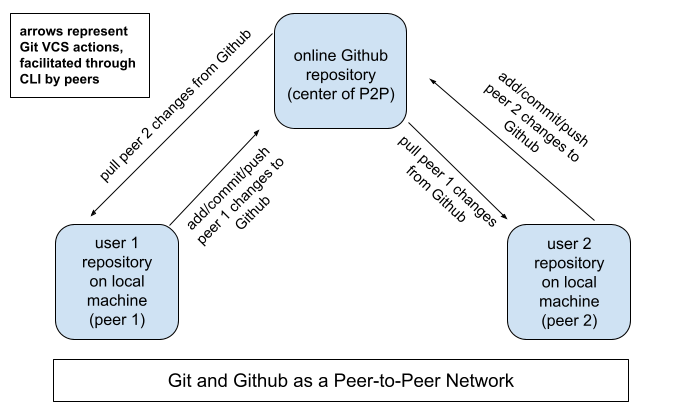
\includegraphics[width=.8\textwidth]{./images/github_p2p_flowchart.png}
\caption{"Flowchart of the P2P circulation of information from user to user on Github."}
\vspace{0in}
\end{center}
\end{figure}
In the flowchart above, the way Git and Github operate as a P2P network is shown. The top of the diagram is the remote repository on Github, which acts as the centralized nature of the system, along with the established Git Flow process of add/commit/push, and lastly the pull of new changes from the remote repository. The lower nodes in the flowchart are the repositories on the local machines of the users, user 1 and user 2, which both represent the peers in the system. To be a peer in this specific system is to be the origin of changes made to the code and information added to the repositories, and facilitating the circulation of information. The sharing of information relies on the actions of the peers. Although not shown the flowchart, the peers will take the decentralized action of adding their own changes in their local repositories. Then, user 1 will use Git send their changes into circulation, carried by Git, through Github, and then to user 2, and vice versa. Through Git and Github, the peers pass information to the other peers in this network. 

Because Git acts as the connecting piece in the P2P system from the peer node to the central server which is Github, and this is how information circulates through the project in the repository and the open source software community of contributors associated with the repository, it is necessary to address what this action means in terms of how Github functions as a library. This P2P system is what characterizes the circulation of information in Github repositories, similar to the circulation of information through physical libraries, but different because this circulation is more decentralized than the physical library. Additionally, peers in the Github P2P system pull or "check out" information through Git from Github, and can also "push" or add the information back into the library system in their new changes format. This is different from checking out a book from the library which is required to be returned in it's original form. Within the Github system, unlike the physical library, it allows for the possibility of discrepancies between local versions of the repository. A contributor could pull the repository and never pull it again while it continues to change on Github. The contributor could also make changes to their local repository which are never pushed to Github. This occurs because Git as a version control system is not automatic, and the user must use it in order for the versions to be recorded on Github. A complication with this specific to Github is how the add/commit/push process can be started, but not finished. For example, the contributor could use git add and leave the process at add, or create the commit and choose not to or forget to push it to Github with git push. 
